\documentclass[12pt, a4paper]{report}
\usepackage[utf8]{vietnam}
\usepackage[top=2cm, bottom=2cm, left=1.5cm, right=1.5cm]{geometry}
\usepackage{amsmath,amsfonts,amssymb}
\usepackage{indentfirst,enumitem}
\usepackage{graphicx}
\usepackage[font=small,labelfont=bf]{caption}
\usepackage{multicol}
\usepackage{setspace}
\usepackage{hyperref}
\usepackage{listings}
\usepackage{tabularx}
\usepackage{hyperref}
\usepackage{xcolor}
\usepackage{scrextend}
\usepackage{comment}
\usepackage{soul}
\usepackage{tikz,tkz-tab}

\renewcommand\thesection{\arabic{section}}
\def \DN {\textbf{Định nghĩa }}

\title{GIẢI TÍCH 2 (CALCULUS 2)}
\author{Vũ Nhật Huy}
\begin{document}
\maketitle
\newpage
\chapter*{ĐẠO HÀM VÀ VI PHÂN NHIỀU BIẾN}
\section{Đạo hàm riêng cấp một.}
Đạo hàm riêng cấp một của $f(x,y)$ theo biến $x$ tại $(x_0,y_0)$: 
\[
    f'_{x}(x_0,y_0)= \frac{\partial f}{\partial x}(x_0,y_0)=\displaystyle\lim_{\Delta x \to 0} \dfrac{f(x_0 + \Delta x,y_0) - f(x_0,y_0)}{\Delta x}  
\]

Đạo hàm riêng cấp một của $f(x,y)$ theo biến $y$ tại $(x_0,y_0)$: 
\[
    f'_{y}(x_0,y_0)= \frac{\partial f}{\partial y}(x_0,y_0)=\displaystyle\lim_{\Delta y \to 0} \dfrac{f(x_0 + \Delta y,y_0) - f(x_0,y_0)}{\Delta y}  
\]

Cố định $y_0$, biểu thức là hàm một biến theo $x$, tính đạo hàm của hàm này tại $x_0$.
\section{Ý nghĩa hình học.}
\begin{center}
    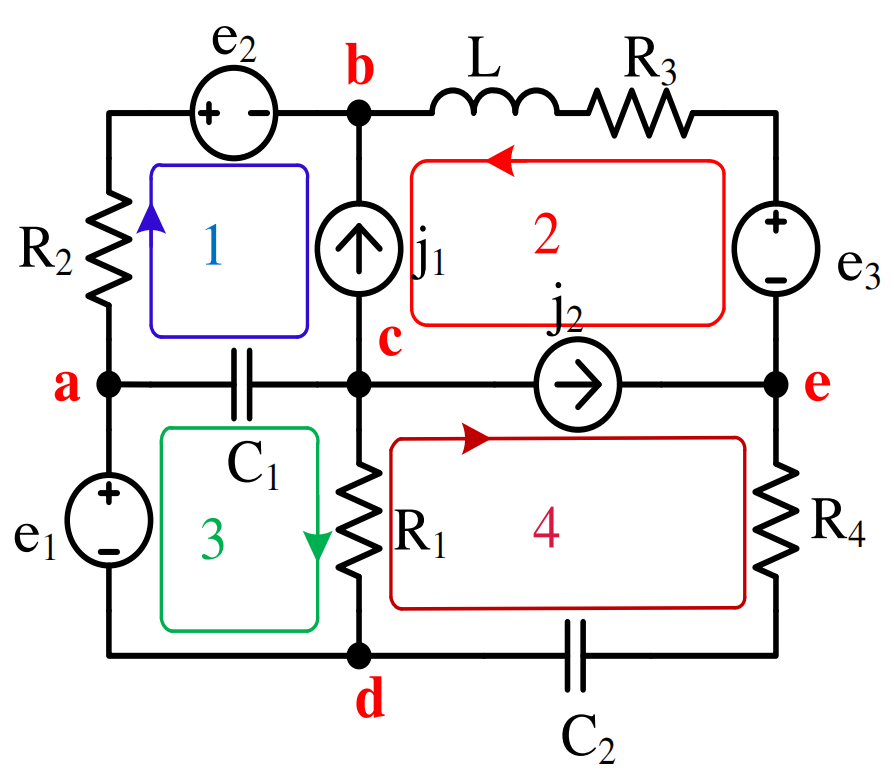
\includegraphics[scale = 0.35]{14.png}
\end{center}
Ý nghĩa hình học của đạo hàm riêng của hàm $f(x,y)$ tại điểm $(x_0,y_0)$ là
\begin{enumerate}
    \item $f'_x(x_0,y_0)$ là hệ số góc của tiếp tuyến $T_1$v với đường cong $C_1$ (trong đó $C_1$ là giao tuyến của mặt cong $S$ với mặt phẳng $y=y_0$)
    \item $f'_y(x_0,y_0)$ là hệ số góc của tiếp tuyến $T_2$v với đường cong $C_2$ (trong đó $C_2$ là giao tuyến của mặt cong $S$ với mặt phẳng $x=x_0$)
\end{enumerate}
\section{Đạo hàm riêng cấp cao.}
Với hàm hai biến $z =f(x,y)$ thì đạo hàm riêng $f_{x}'$ và $f_{y}'$ cũng là những hàm hai biến, do đó những đạo hàm riêng của chúng $(f_{x}')_{x}'$, $(f_{x}')_{y}'$, $(f_{y}')_{x}'$, $(f_{y}')_{y}'$ được là đạo hàm riêng cấp hai của hàm $f$. Như vậy:
\[
  \frac{\partial}{\partial x}\left( \frac{\partial f}{\partial x}\right) = \frac{\partial^2 f}{\partial x^2} = f_{xx}''; \thickspace \frac{\partial}{\partial y}\left( \frac{\partial f}{\partial x}\right) = \frac{\partial^2 f}{\partial x \partial y} = f_{xy}''
\]
\[
  \frac{\partial}{\partial x}\left( \frac{\partial f}{\partial y}\right) = \frac{\partial^2 f}{\partial y \partial x} = f_{yx}''; \thickspace \frac{\partial}{\partial y}\left( \frac{\partial f}{\partial y}\right) = \frac{\partial^2 f}{\partial y^2} = f_{yy}''    
\]
\textbf{\textit{Định lý Clairaut (Schwartz).}} Cho hàm số $z =f(x,y)$ xác định trên miền $D$. Khi đó  nếu $f_{xy}''$ và $f_{yx}''$ là những hàm liên tục trên $D$ thì với mọi $(x_0,y_0) \in D$ ta có $f_{xy}'' (x_0,y_0) = f_{yx}'' (x_0,y_0)$.
\section{Sự khả vi và vi phân cấp một}
%\[
%\begin{aligned}
%    &\lim_{x \to + \infty} \left( \sqrt[3]{x^3 + 2x^2} - \sqrt{x^2 - 2x} \right)  \\
%    = &\lim_{x \to +\infty} \left\lbrack \left( \sqrt[3]{x^3 + 2x^2} -x \right) + \left(x- \sqrt{x^2 - 2x} \right) \right\rbrack  \\
%    = &\lim_{x \to +\infty} \frac{\left( \sqrt[3]{x^3 + 2x^2} -x \right)\left( \sqrt[3]{x^3 + 2x^2} +x \right)^2}{(\sqrt[3]{x^3 + 2x^2} +x)^2} + \lim_{x \to +\infty} \frac{\left(x- \sqrt{x^2 - 2x} \right)\left( x+\sqrt{x^2 - 2x} \right)}{x+ \sqrt{x^2 - 2x}}
%\end{aligned}    
%\]
$f$ khả vi tại $(x_0,y_0)$ nếu tồn tại hai hằng số $A,B$ sao cho: 
\[
    f(x_0,\Delta x,y_0 + \Delta y) - f(x_0,y_0) = f'_x (x_0,y_0)\Delta x + f'_y (x_0,y_0)\Delta y + o\left( \sqrt{\Delta x^2 + \Delta y^2}\right)
\]
Điều kiện cần của khả vi: 
\begin{enumerate}
    \item $f$ khả vi tại $(x_0,y_0)$ thì $f$ liên tục tại $(x_0,y_0)$.
    \item $f$ khả vi tại $(x_0,y_0)$ thì $f$ có các đạo hàm riêng tại $(x_0,y_0)$.
\end{enumerate}
Vi phân của hàm hai biến thường viết dưới dạng:
\[
    df(x_0,y_0)=f'_x (x_0,y_0)dx + f'_y (x_0,y_0)dy    
\]
Điều kiện đủ của khả vi: Cho $f$ xác định trong miền mở chứa $(x_0,y_0)$, nếu các đạo hàm riêng $f'_x,f'_y$ liên tục tại $(x_0,y_0)$ thì $f$ khả vi tại $v(x_0,y_0)$.
\section{Vi phân cấp cao.}
Vi phân cấp hai của $f$ là vi phân của $df(x,y)$ khi xem $dx,dy$ là các hằng số. Cách viết: $d^2 f(x,y)=d(df(x,y))$.
\[
    d^2 f(x,y) = f_{xx}''dx^2 + 2f_{xy}''dxdy + f_{yy}''dy^2
\]
Công thức trên áp dụng khi $x,y$ là các biến độc lập.\\
Công thức tổng quát cho vi phân cấp cao.
\[
    d^n f(x,y) = \left( \frac{\partial}{\partial x}dx + \frac{\partial}{\partial y}dy \right)^n f(x,y)    
\]
\section{Đạo hàm và vi phân của hàm hợp.}
Cho $z = f(x,y)$ và $x=x(u,v), y=y(u,v)$. Nếu $z,x,y$ khả vi:
\[
    z_u '= f'_x.x'_u + f'_y.y'_u \qquad z_v '= f'_x.x'_v + f'_y.y'_v
\]
\[
    \begin{aligned}
        &dz = z'_u du + z'_v dv \\
        &df = f'_x du + f'_y dv = (f'_x.x'_u + f'_y.y'_u)du + (f'_x.x'_v + f'_y.y'_v)dv\\
        &df = f'_x(x'_u du + x'_v dv) + f'_y(y'_u du + y'_v dv)   
    \end{aligned}    
\]

\textbf{Trường hợp riêng 1.} Cho $z = f(x)$ và $x = x(u,v)$ (hợp của 1 biến và 2 biến).
\[
    z'_u = f'(x)x'_u \qquad z'_v = f'(x)x'_v    
\]
\[
    \begin{aligned}
        &dz = z'_u du + z'_v dv \\
        \Longrightarrow &dz = f'(x)dx = f'(x)(x'_u du + x'v dv)
    \end{aligned}    
\]

\textbf{Trường hợp riêng 2.} $z = f(x,y), x = x(t), y = y(t)$ (hợp 2 biến và 1 biến).
\[
    z'(t) = f'_x.x'(t) + f'_y.y'(t)   
\]
\[
    \begin{aligned}
        &dz = z'(t) dt \\
        &dz = f'_x dx + f'_y dy = f'_x.x'(t) dt + f'_y.y'(t) dt
    \end{aligned}
\]

\textbf{Trường hợp riêng 3.} $z=f(x,y), y= y(x)$ (hợp 2 biến và 1 biến).
\[
    z'(x) = f'_x + f'_y.y'(x)    
\]
\[
    dz = z'(x) dx    
\]
\textcolor{red}{\textbf{Lưu ý:}} Khi tính đạo hàm hàm hợp, luôn bắt đầu từ  đạo hàm của $f$ theo biến chính. Sau đó, tùy thuộc vào yêu cầu, nhân thêm đạo hàm của biến chính vào cạnh đạo hàm của $f$.
\section{Đạo hàm và vi phân hàm ẩn.}
$G = F(x,y) = 0$, với $y=y(x)$. Đạo hàm của hàm ẩn 1 biến $y=y(x)$ (Xem $x,y$ là hai biến độc lập khi lấy đậo hàm của $F$):
\[
    y'(x) = \frac{-F'_x}{F'_y}    
\]

Xét hàm ẩn 2 biến $z=z(x,y)$ xác định từ phương trình $F(x,y,z) = 0$ ($x,y,z$ là các biến độc lập khi tính $F'_x,F'_y,F'_z$)
\[
    z'_x = \frac{-F'_x}{F'_z}, \qquad z'_y = \frac{-F'_y}{F'_z}
\]
\subsection{Phương trình tiếp tuyến.}
Cho đường cong $C$ được xác định bởi $F(x,y) = 0,\thickspace P(x_0,y_0) \in C$. Khi đó phương trình tiếp tuyến với đường cong $C$ tại điểm $P$ là: 
\[
    F'_x(x_0,y_0)(x-x_0) + F'_y(x_0,y_0)(y-y_0) = 0
\]
\subsection{Mặt phẳng tiếp diện.}
Cho mặt cong $S$ được xác định bởi $F(x,y,z) = 0,\thickspace P(x_0,y_0,z_0)$. Khi đó phương trình mặt phẳng tiếp diện với mặt cong $S$ tại điểm $P$ là:
\[
    F'_x(x_0,y_0,z_0)(x-x_0) + F'_y(x_0,y_0,z_0)(y-y_0) + F'_z(x_0,y_0,z_0)(z-z_0) = 0
\]
\section{Đạo hàm theo hướng.}
Cho $f(x,y)$ là hàm khả vi và có đạo hàm theo hướng của véc-tơ đơn vị $u=(a,b), (a^2 + b ^2 = 1)$. Khi đó:
\[
    f'_{\Vec{u}} (x,y) = f'_x (x,y).a + f'_y (x,y).b    
\] 
Ý nghĩa hình học: Đạo hàm theo hướng là hệ số góc của tiếp tuyến đối với đường cong tại 1 điểm.
\subsection{Véc-tơ Gradient.}
Cho $z=f(x,y)$, khi đó véc-tơ gradient của hàm số $f$ được xác định như sau:
\[
    \bigtriangledown f(x,y) = (f'_x (x,y),f'_y (x,y))
\]

Cho $z=f(x,y),u=(a,b), (a^2 + b ^2 = 1)$. Khi đó:
\[
    f'_{\Vec{u}} (x,y) = < \bigtriangledown f(x,y),u > \qquad (\text{tích vô hướng})
\]
\subsection{GTLN, GTNN của đạo hàm theo hướng.}
Cho $f$ là hàm khả vi 2 hoặc 3 biến. GTLN của đạo hàm theo hướng $\Vec{u}$: $f'_{\Vec{u}}$ là $|\bigtriangledown f|$ đạt được khi $\Vec{u} \uparrow \uparrow \bigtriangledown f$. GTNN của đạo hàm theo hướng $\Vec{u}$: $f'_{\Vec{u}}$ là $-|\bigtriangledown f|$ đạt được khi $\Vec{u}$ ngược hướng $\bigtriangledown f$.
\end{document}